\section{TRABAJO ENCARGADO} 

EL Área de Marketing ha recolectado una lista de 1000 Clientes potenciales y 300 de ellos han comprado algunos de nuestros productos, y los vendedores lo han registrado en Excel, igual forma los registros en Excel de las ordenes y sus detalles de ventas.
El Gerente de Marketing quiere que sean cargados al Sistema en un tiempo corto de horas, Los técnicos siempre lo cargan usando la interface del sistema, y siempre demoran entre 3 dias y cometen ciertos errores al digitar.
y se ha vuelto costumbre que los técnicos lo hagan todo a mano.
Entonces el Gerente de Marketing recurre a Sector de TI para que ellos brinden alguna alternativa de procesamiento rápido, eficaz, y con un riesgo muy bajo de errores.
Se sabe que los vendedores que recolectan estos datos no siempre entregan todo bien Limpio, normalizado.
Marketing tiene asignado un directorio donde están copiando los archivos.

\begin{itemize}
    \item \textbf{GENERAR ARCHIVOS EN EXCEL PARA CUSTOMER y diseñar un ETL para la carga automática.}

En muchas oportunidades, en proyectos donde se tienen que trasladar archivos a un reporsitorio sea del usuario final o sea que el usuario deja compartido, y se tiene que procesar para cargarlo al sistema o aun Data Warehouse, en SSIS se cuenta con la funcionalidad de desarrollar esto.

ESTRUCTURA DE CONTROL FLOW: FUNCIONALIDAD (Manipulación, Mover, Renombrar el Archivo)

	\begin{center}
	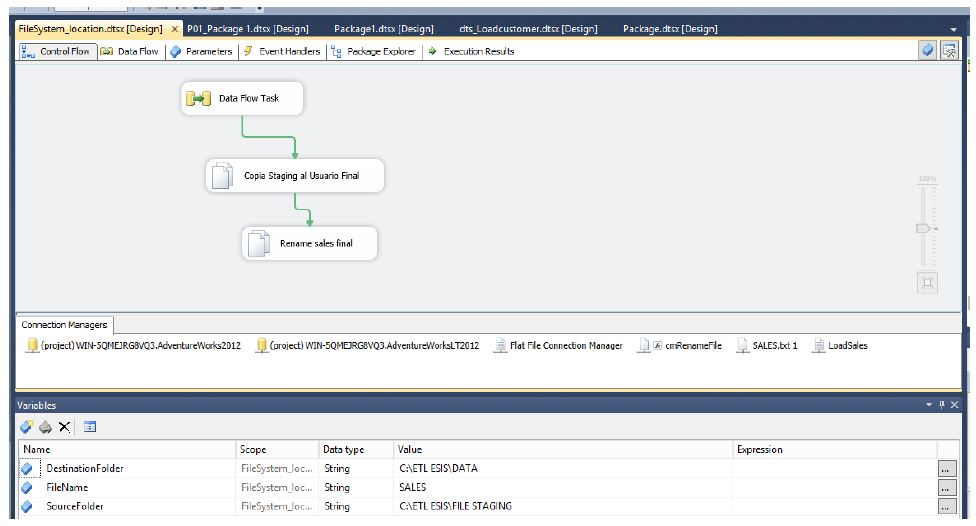
\includegraphics[width=17cm]{./Imagenes/26}
	\end{center}	

- Desarrollo de: Data Flow Task.

	\begin{center}
	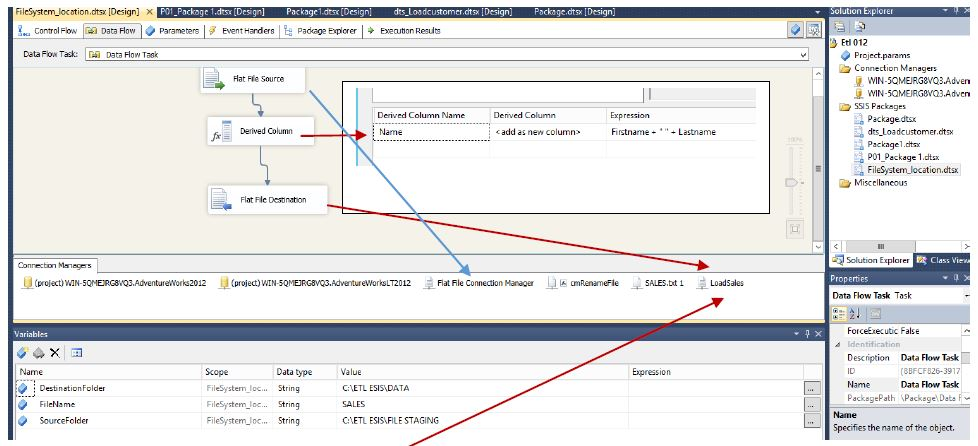
\includegraphics[width=17cm]{./Imagenes/27}
	\end{center}	

    \item \textbf{CREACION DE NEW FILE CONECCION}

	\begin{center}
	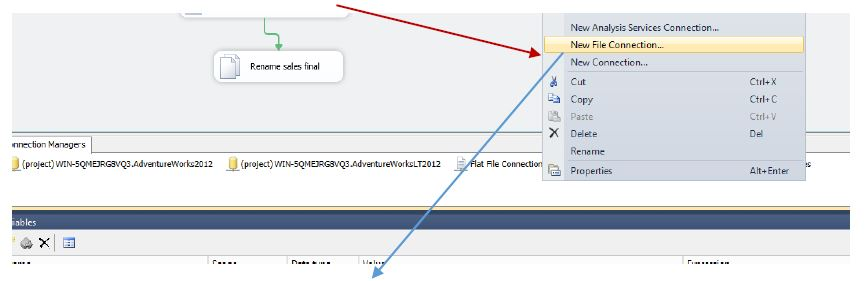
\includegraphics[width=17cm]{./Imagenes/28}
	\end{center}	

	\begin{center}
	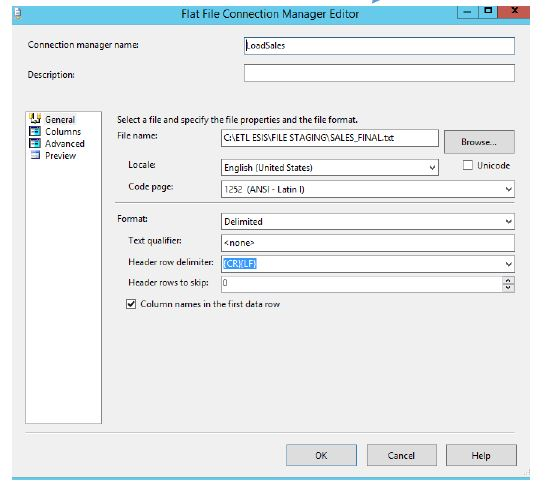
\includegraphics[width=14cm]{./Imagenes/29}
	\end{center}	

- Configuramos el Path de cmRenameFile. Usando expresiones y variables.

	\begin{center}
	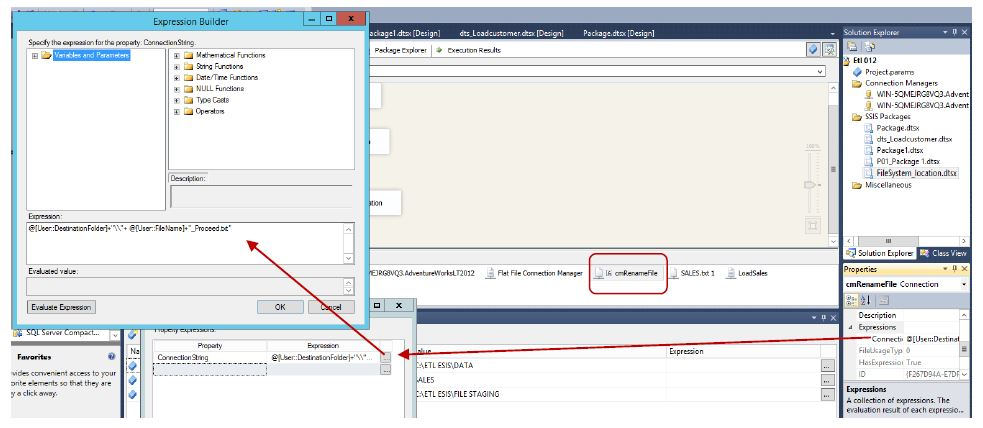
\includegraphics[width=17cm]{./Imagenes/30}
	\end{center}	

-Los procesos ETL deben ser capaz de copiar los archivos a su Espacio Staging para desde ahí realizar la carga al SSIS, Limpiarla y darle formato para cargarlo a la tabla objetivo.
\end{itemize}